% generated by make_figs.py -- do not edit by hand
\begin{figure*}[t]
\centering
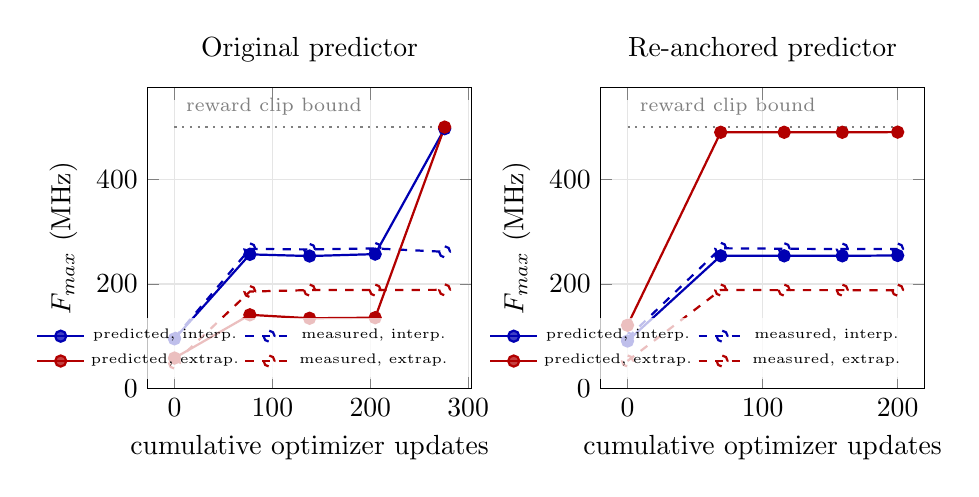
\begin{tikzpicture}

\begin{axis}[
  name=v8, title={Original predictor},
  width=.47\textwidth, height=5.4cm,
  xlabel={cumulative optimizer updates},
  ylabel={$F_{max}$ (MHz)}, ymin=0, ymax=575,
  legend pos=south east, legend columns=2,
  legend style={font=\tiny, draw=none, fill opacity=.75, text opacity=1},
  grid=major, grid style={gray!20}
]
\addplot[gray, dotted, thick, forget plot] coordinates {(0,500) (276,500)};
\node[gray, font=\scriptsize, anchor=south west] at (axis cs:2,503) {reward clip bound};

\addplot[blue!70!black, mark=*, thick] coordinates {(0.0,95.1) (77.0,256.6) (138.0,253.4) (205.0,257.1) (276.0,496.9)};
\addlegendentry{predicted, interp.}
\addplot[blue!70!black, mark=o, thick, dashed] coordinates {(0.0,96.6) (77.0,267.1) (138.0,266.0) (205.0,267.9) (276.0,261.5)};
\addlegendentry{measured, interp.}

\addplot[red!70!black, mark=*, thick] coordinates {(0.0,58.3) (77.0,141.0) (138.0,134.4) (205.0,135.5) (276.0,500.0)};
\addlegendentry{predicted, extrap.}
\addplot[red!70!black, mark=o, thick, dashed] coordinates {(0.0,48.8) (77.0,185.5) (138.0,188.3) (205.0,188.3) (276.0,188.8)};
\addlegendentry{measured, extrap.}
\end{axis}
\begin{axis}[
  at={(v8.right of south east)}, xshift=13mm, ylabel={}, title={Re-anchored predictor},
  width=.47\textwidth, height=5.4cm,
  xlabel={cumulative optimizer updates},
  ylabel={$F_{max}$ (MHz)}, ymin=0, ymax=575,
  legend pos=south east, legend columns=2,
  legend style={font=\tiny, draw=none, fill opacity=.75, text opacity=1},
  grid=major, grid style={gray!20}
]
\addplot[gray, dotted, thick, forget plot] coordinates {(0,500) (200,500)};
\node[gray, font=\scriptsize, anchor=south west] at (axis cs:2,503) {reward clip bound};

\addplot[blue!70!black, mark=*, thick] coordinates {(0.0,90.9) (69.0,253.8) (116.0,253.8) (159.0,253.8) (200.0,254.5)};
\addlegendentry{predicted, interp.}
\addplot[blue!70!black, mark=o, thick, dashed] coordinates {(0.0,96.7) (69.0,268.2) (116.0,267.4) (159.0,266.7) (200.0,266.7)};
\addlegendentry{measured, interp.}

\addplot[red!70!black, mark=*, thick] coordinates {(0.0,121.0) (69.0,490.1) (116.0,490.1) (159.0,490.1) (200.0,490.4)};
\addlegendentry{predicted, extrap.}
\addplot[red!70!black, mark=o, thick, dashed] coordinates {(0.0,52.8) (69.0,188.4) (116.0,188.2) (159.0,188.2) (200.0,188.1)};
\addlegendentry{measured, extrap.}
\end{axis}
\end{tikzpicture}
\caption{Predicted and measured \fmax{} along the optimisation path, for the
twelve held-out \textsc{fir}/\textsc{firr} designs ($n{=}16$ samples each),
count-weighted over correct candidates. The abscissa is cumulative optimizer
updates rather than attempted steps, because a group whose rewards are all equal
yields no gradient and the two runs differ in how often that happens.
\textbf{Left:} under the original predictor, prediction tracks measurement on
the interpolation designs to within $12$\,MHz for roughly two hundred updates and
then saturates at the reward's clip bound ($496.9$ predicted against $261.5$
measured), while on the extrapolation designs it first \emph{under}-predicts and
then saturates as well. Note what measurement does \emph{not} do: conditional on
correctness it is flat from the first checkpoint onward, so saturation does not
make the policy's correct outputs slower. What it does is stop penalising the
incorrect ones---correctness falls at exactly the saturating checkpoint, and
falls where the saturation is worst ($92.2\%\!\to\!73.4\%$ on extrapolation
against $96.9\%\!\to\!95.3\%$ on interpolation). \textbf{Right:} after re-anchoring on
$43$ train-split measurements, the interpolation curves stay together for the
whole run ($254.5$ against $266.7$ at the end) and no collapse occurs. The
extrapolation curves do not recover: the re-anchor labels span $4$--$32$ taps, so
at $36$ and $40$ taps the predictor is pinned near the clip bound from the first
checkpoint onward and orders nothing. Measured extrapolation frequency is
consequently the same under both rewards ($188.8$ against $188.1$); the
improvement the repair buys is confined to the region the labels reach. We read
this as the sharper form of the claim -- a learned reward is valid only over the
support of its supervision, and offline accuracy reports nothing about the region
optimisation will travel to.}
\label{fig:trajectory}
\end{figure*}
